\chapter{Démarche adoptée et réalisations au sein de PPIL}
\label{chap:premierchapitre}

% --> A ajouter : 
% présentation de PPIL
% indicateurs intéressants. dans montée en compétence : Un projet de gestion de projet
% retour PMO
% mieux rédiger TNR
% mieux rédiger ANO
% vu toute la production d'un projet
%CNAM Métier
%HP ALM

\section{Montée en compétence sur le fonctionnel du projet}

Pendant ma première semaine de stage, j'ai effectué une montée en compétence sur le fonctionnel du projet. Il est important de souligner que j'ai continué à en apprendre toujours d'avantage sur le fonctionnel du projet tout le long de mon stage, que ce soit en qualification ou en développement.

Il est évident que cette montée en compétence a été primordiale pour la suite de mon stage. Dans cette section, je vais décrire ma démarche pour m'imprégner du projet. Pour cela, j'ai utilisé plusieurs méthodes :

Tout d'abord, j'ai étudié les spécifications fonctionnelles et techniques du projet (SFG, SFD et STD), je me suis aussi procuré le manuel utilisateur de l'application auprès de l'équipe.

Au cours de cette montée en compétence, j'ai posé des questions aux différents analystes fonctionnels du projet. J'ai donc pu bénéficier de leurs explications.

Quelques informations importantes que j'ai pu recueillir lors de mon arrivée dans l'équipe :
\begin{itemize}
    \item Début de PPIL en 2010 ;
    \item Refonte du projet en 2017 ;
    \item Exigences du client ;
    \item Des sprints qui durent 3 semaines ;
    \item Les besoins et les outils du client (les différents acteurs de la CNAM utilisent MSP) ;
    \item Comprendre les différentes fonctionnalités de PPIL ;
    \item PPIL et les autres projets de la CNAM : on retrouve dans PPIL tous les autres projets de la CNAM ;
    \item PPIL est intégré dans SharePoint dans le but d'avoir une meilleure organisation interne ;
    \item Fonctionnement du Reporting de PPIL ;
    \item Différents concepts : indicateurs, jalons, diagrammes, lots, projet de référence, projets contributeurs ; 
\end{itemize}

En plus de ces explications et cette étude des documents, j'ai pu manipuler l'application PPIL, la prendre en main afin de me mettre à la place des utilisateurs finaux et de comprendre comment et pourquoi ils utilisent cet outil qu'est PPIL.

A la fin de la semaine, j'ai réalisé une présentation du projet et de ses fonctionnalités aux membres de mon équipe. La présentation a duré dix minutes. Cette présentation a eu pour objectif de présenter tout ce que j'ai appris sur le projet durant la semaine. A la suite de cette présentation, nous avons échangé avec les BA, RT et le chef de projet afin de préciser certains points importants dans l'objectif d'en savoir un maximum sur le projet.

\subsection{Des indicateurs intéressants en terme de gestion de projet}

Il est évident que PPIL est très intéressant en terme de gestion de projets. Il permet de voir comment une organisation (la CNAM) gère une multitude de projets. Et aussi de voir comment sont gérés les différentes phases d'un projet.

J'ai découvert dans PPIL le mécanisme de reporting de projets et de lots ainsi que des indicateurs qui permettent de :
\begin{itemize}
    \item Planifier les projets dans le temps (notamment grâce aux concepts de jalons) ;
    \item Maîtriser et piloter les risques ;
    \item Gérer un grand nombre de projets ;
    \item Suivre des enjeux opérationnels de projets ou de lots ;
    \item S'adapter en fonction des différents acteurs intervenants dans la gestion de projets.
\end{itemize}
\vspace{\baselineskip}
L'objectif dans cette partie est de présenter \textbf{quelques indicateurs} visibles dans PPIL. C'est un portail qui est peut être en phase de devenir \textbf{une référence en terme de gestion de projets}. A fortiori pour moi, étudiant en informatique. 

\subsubsection{Quelques indicateurs}

PPIL permet aux différents profils d'utilisateurs de visualiser les informations opérationnelles de leurs projets.

Pour les profils Chef de projet, Manager, Responsable DSI et MOA, on peut :
\begin{itemize}
    \item Visualiser l’indicateur \textbf{Bulletin de santé} : les projets dont la tendance est en dégradation et/ou la météo est orageuse sont mis en évidence par cet indicateur ;
    %\item Visualiser l’indicateur \textbf{Dérive des jalons}
    %\begin{itemize}
        %\item Les projets dont le prochain jalon et/ou la date de mise en production est en dérive sont mis en évidence par cet indicateur.
        %\item Un jalon est en dérive lorsqu’il existe une différence de plus de 7 jours entre les dates du dernier reporting et de celui fait il y a un mois.
    %\end{itemize}
    \item Visualiser l’indicateur \textbf{Avancement par phase} (Chef de projet) : les jalons de tous les projets aux états « En cours » du périmètre sont représentés dans cet indicateur ;
    \item Visualiser l’indicateur Plan de charge équipe (Manager) ;
    %En cliquant sur le graphique, on accède au rapport du Capacity Planning
    %\item Visualiser l’indicateur \textbf{Planning des MEP} (mise en production) : Responsable DSI et MOA
    %Les lots dont la date de mise en production est comprise entre le mois passé et les six prochains mois sont placés sur une échelle de temps.
\end{itemize}

\begin{figure}[h]
\centering
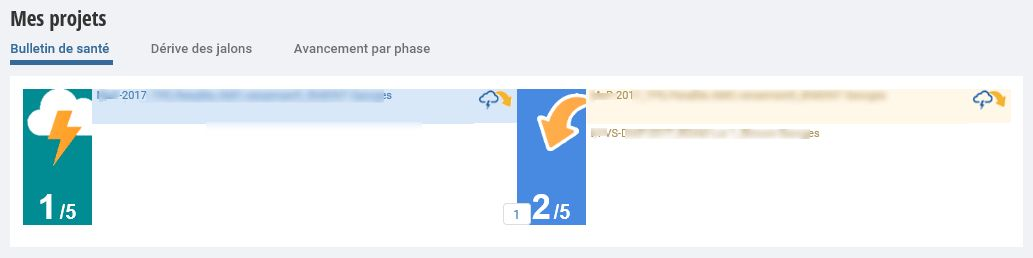
\includegraphics[width=1\textwidth]{images/ppil-bulletion-de-sante-censored.png}
\caption{PPIL : Bulletin de santé (Profil Chef de Projet)}
\end{figure}

\subsubsection{Accéder aux reporting / restitution d'un lot / projet}

Pour rappel, un lot contient plusieurs projets. En cliquant sur le nom d’un projet/lot, les indicateurs s'affichent soit en saisie, soit en restitution, en fonction des profils. 

En accédant au reporting d'un projet, on accède à différents indicateurs intéressants pour un lot/projet : 

Ci-dessous on peut retrouver l'avancement par phases des projets d'un lot ainsi que détail de toutes les phases de réalisation des projets. On peut voir l'évolution de chacun d'eux (en haut on peut voir le projet de référence).

\begin{figure}[h]
\centering
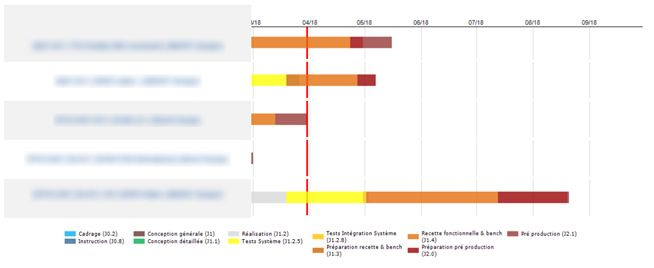
\includegraphics[width=1\textwidth]{images/PPIL-Gantt-censored.png}
\caption{PPIL : Diagramme de Gantt / Avancement par phase}
\end{figure}

Ci-dessous on peut visualiser l'avancement en charges qui nous donne des indicateurs de performance d'un lot (c'est à dire un ensemble de projet) : on peut noter que l'indicateur "avancement en charges" est calculé à partir du "consommé global" et du "RAF". Le Forecast est calculé à partir du : "Consommé global", du "RAF" et des Charges. J'ai du vérifier tous les indicateurs du graphique d'avancement en charges lors d'une des phases de qualification (pendant les tests de non régression).
\begin{figure}[h]
\centering
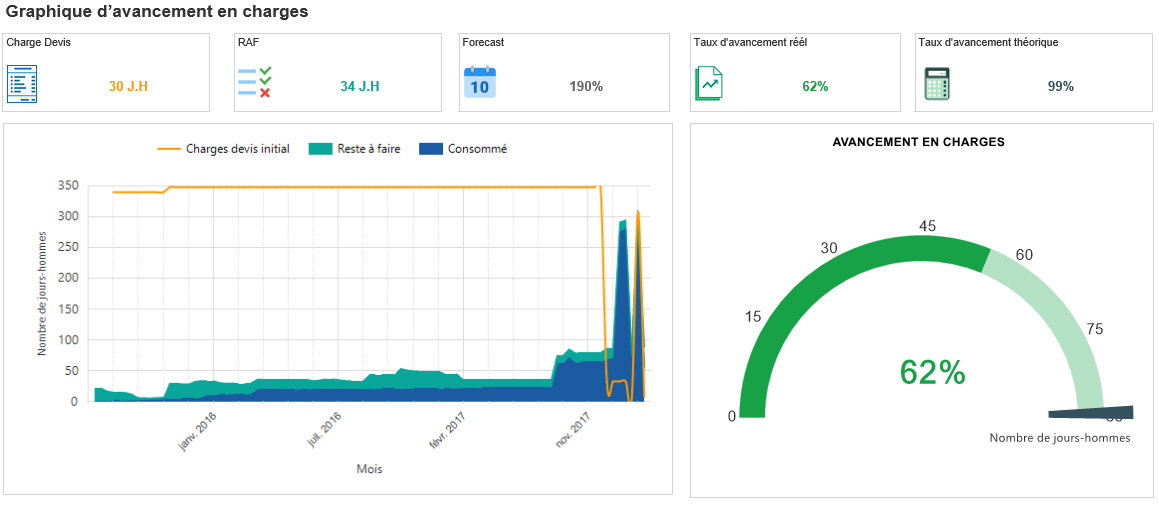
\includegraphics[width=1\textwidth]{images/PPIL-avancement.png}
\caption{PPIL : Graphique d'avancement en charges}
\end{figure}

L'indicateur ci-dessous précise l'avancement d'un projet en fonction des différents jalons. On peut voir les jalons dont la date a été franchie, reportée ou en retard. 

\begin{figure}[H]
\centering
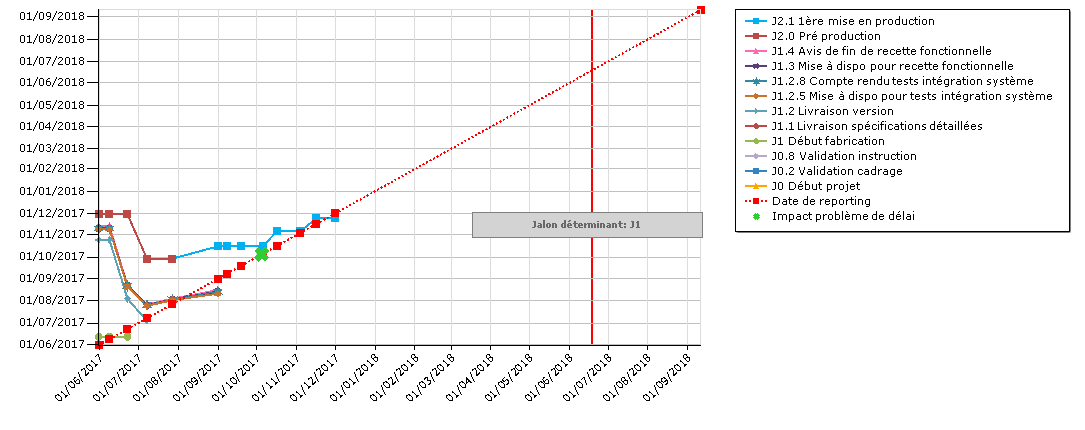
\includegraphics[width=1\textwidth]{images/temps-temps.png}
\caption{PPIL : Diagramme temps-temps}
\end{figure}

\section{La qualification}

Une partie de mon stage est destinée à la qualification. J'ai effectué différents tests :
\begin{itemize}
    \item Tests fonctionnels ; 
    \item Tests de Non Régression ;
    \item Plan de tests ;
\end{itemize}

\subsection{L'importance des tests}

J'ai réalisé des tests afin de vérifier le bon fonctionnement des nouvelles fonctionnalités. Ainsi que des corrections du projet ayant pour objectif de détecter d'éventuels anomalies ou régressions. Ces tests m'ont étés bénéfiques pour comprendre PPIL en profondeur. En effet, pour chaque test, il faut comprendre et manipuler la base de données du projet, consulter les spécifications techniques ou fonctionnelles (SFG, STD) et poser des questions aux différents membres de l'équipe.

Au cours de ces tests, j'ai rencontré plusieurs difficultés : 

\begin{itemize}
    \item Certaines fonctionnalités à tester ne sont pas évidentes à comprendre ou à reproduire.
    \item Les principes de l'outil (par exemple la logique de reporting en fonction des différents indicateurs).
    \item Manipuler une base de données complexe (préparer des jeux de données, changer d'utilisateur, vérifier des informations en base).
\end{itemize}

A chaque fois, ces tests ont été effectués avant une livraison interne ou une livraison client.

Lors des tests, il est important de prendre du recul et de tester d'autres fonctionnalités. Le portail pourrait être impacté par la correction qu'on est en train de tester. Tous ces tests ont été réalisé grâce à l'outil HPALM.
        
Valider un test c'est prendre la responsabilité de dire qu'on peut livrer l'application. L'étape du test est primordiale. Sans celle-ci un bon nombre d'erreurs ne seraient pas détectées.

\subsection{Les plans de tests}

J'ai eu l'occasion de rédiger des plans de tests. Cette étape demande une grande rigueur car il est important de couvrir tout le périmètre de la fonctionnalité à tester pour découvrir d'éventuelles régressions. Ci-dessous, un exemple de plan de test :

\begin{figure}[!h]
\centering
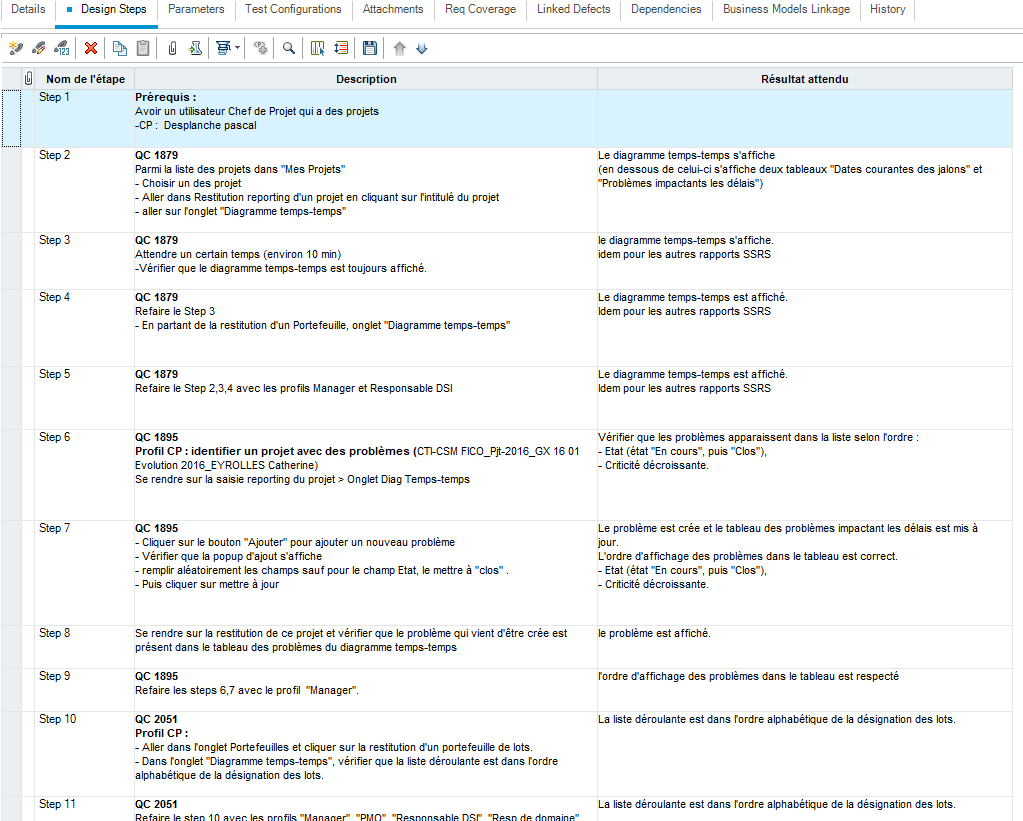
\includegraphics[width=0.8\textwidth]{images/HPLMplantest.png}
\caption{HPALM : Un plan de test}
\end{figure}

\subsection{Un exemple de test réalisé : Les tests de Non Régression (TNR)}

Avant la livraison de la release 20.06.00. Il a fallu effectuer des tests de non régression.

Je vais décrire ici le test "06-TNR-ReportingRestitutionDuLot". Lors de ce test, j'ai détecté trois Defects. Ce qui a permis d'identifier et corriger une anomalie mineure, une anomalie majeure, et une régression majeure. Au cours de ce test de 40 steps, j'ai effectué un grand nombre de requêtes SQL. J'ai dû comprendre la logique de calcul ainsi que la logique d'affichage des indicateurs d'avancement d'un projet en fonction des jalons de celui-ci. Il a fallu que j'analyse la synchronisation des données projet entre Microsoft Project et PPIL.

\subsubsection{Difficultés rencontrées lors de ce test}

\textbf{Description d'une étape qui m'a posée des difficultés pendant ce test :}
C'est l'étape de vérification des indicateurs de suivi d'avancement du lot que j'ai choisi de détailler.
Le cas à vérifier se trouve dans PPIL, dans la partie restitution de l'avancement d'un projet de référence. Mon but étant de vérifier que les résultats restitués dans les indicateurs soient bien correct. Pour cela il a fallu que j'aille chercher les données en base et que j'effectue des calculs avec ces données.
Pour comprendre comment sont calculés les indicateurs de restitution pour l'avancement d'un lot, j'ai consulté les SFD afin de récupérer les règles de calcul. Je suis allé en base de données afin de récupérer les données (récupérer les projets à partir desquels les calculs sont effectués). J'ai du faire des requêtes assez complexes pour récupérer les bons projets. Après cela, j'ai importé les projets et leurs informations dans Excel pour y faire mes calculs. N'ayant toujours pas le bon résultat, mais ayant fait ces calculs avec rigueur, j'ai demandé des explications à un BA, notamment, sur un détail fonctionnel particulier. Ce détail portait sur la synchronisation des données de Microsoft Project dans PPIL (outil utilisé par les Chef de projet de la CNAM pour mettre à jour les jalons de leurs projets). J'ai finalement trouvé la solution. Grâce aux explications et à l'analyse d'une procédure stockée.

%Pour résumer, j'ai du faire appel à plusieurs
%Expliquer ce problème
%De restitution qui importe les projets contributeurs (qui font parti du même PRT Palier).
%Pour la partie Avancement en charge
\begin{figure}[h]
\centering
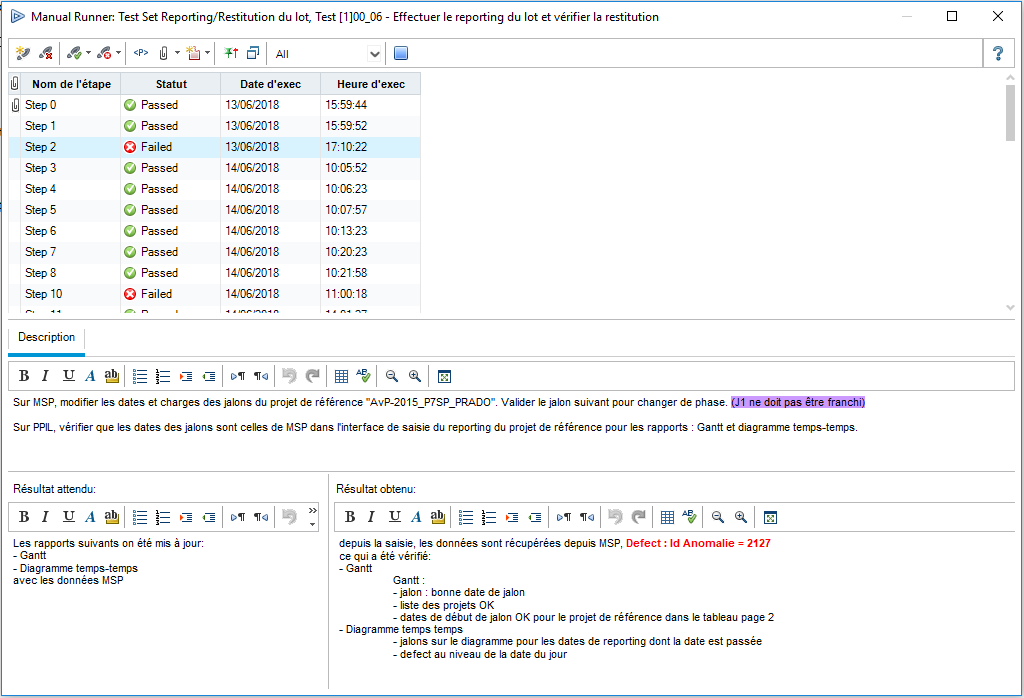
\includegraphics[width=0.8\textwidth]{HPALM-test.PNG}\\[1cm]
\caption{HPALM : Déroulement d'un test}
\end{figure}

\section{Environnement technique du projet}

Pendant la deuxième semaine, j'ai également mis en place mon environnement de développement avec Achref (mon SB référent). Le projet PPIL se situe dans un contexte technique Microsoft : 

\begin{itemize}
    \item Sharepoint, 
    \item SQLServer, 
    \item .Net
    \begin{itemize}
        \item C\#, 
        \item Telerik, 
        \item TypeScrypt, 
        \item Entity Framework, 
        \item SSRS, 
        \item HTML, 
        \item CSS.
    \end{itemize}
\end{itemize}

Outils utilisés :
\begin{itemize}
    \item Visual Studio,
    \item HPALM,
    \item Git,
    \item Microsoft SQL Server Management,
    \item Microsoft Team Foundation Server.
\end{itemize}

\section{Développer au sein de PPIL}

J'ai commencé à développer au mois de Mai. Les développements au sein de PPIL se font en fonction de l'évolution du sprint en cours. Je suis arrivé dans un contexte de corrections d'anomalies. C'est naturellement que des (QC) corrections d'anomalies m'ont été attribuées.

Ma première tâche a été de normaliser la charte graphique en même temps que l'interface du projet dans le but d'harmoniser les deux. Cette tâche fait suite à un retour du client (FT). Cela m'a permis de découvrir l'environnement technique. 

Ensuite, j'ai principalement corrigé des anomalies et développé quelques évolutions.

\subsection{Corrections d'anomalies}

Lorsque les BA détectent une anomalie, ils l'identifient et la répertorie dans l'outil HPALM. Il est important de préciser que certaines anomalies sont détectées par le client. Elles sont classées par priorité et importance.
Les FT (anomalie retour client) sont souvent prioritaires par rapport aux anomalies détectées par l'équipe.
Un lot correspond à une version de l'application, chaque anomalie est rattaché à un lot.

\begin{figure}[h]
\centering
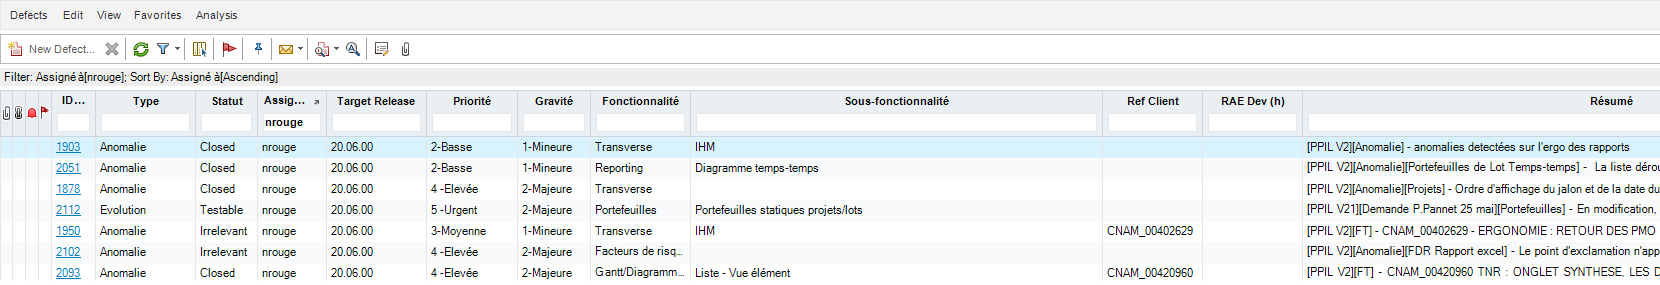
\includegraphics[width=0.8\textwidth]{images/HPLMliste.png}
\caption{HPALM : Anomalies corrigées de la release 20.06.00}
\end{figure}

\subsection{Démarche Adoptée}

Avant de commencer le développement, j'ai dû lire les consignes de code, règles à respecter soigneusement car mes développements seront livrés directement.

J'ai été chargé de corriger les anomalies distribuées par les RT.
Le référent technique a attribué différentes QC (Anomalies) aux différents SB. 
Les anomalies que j'ai corrigées étaient toutes différentes et incluaient différentes technologies à chaque fois.

Quelques exemples d'anomalies que j'ai corrigées : 
\begin{itemize}
    \item Suppression d'un élément qui ne se supprime pas en base ;
    \item Erreur dans le chargement d'une page ;
    \item Bouton "annuler" non présent ;
    \item Ordre ou classement incorrect ;
    \item Re-direction de page incorrecte lors de la consultation...
\end{itemize}

Pour mener à bien ces différentes corrections, il a été important de prendre du recul avant chaque correction. De bien identifier le périmètre de l'anomalie afin d'éviter les régressions.

Tout d'abord, j'ai du comprendre et analyser l'architecture du programme afin d'identifier plus facilement la provenance des anomalies. 

Chacun des points suivants ont été très importants dans ma démarche de correction d'anomalies :
\begin{itemize}
    \item Étudier l'architecture de la base de données a été primordial pour avoir une visibilité sur les relations entre les différentes entités ;
    \item Me former sur les technologies ;
    \item Comprendre l'anomalie aussi bien fonctionnement que techniquement ;
    \item Analyser l'ampleur et le périmètre de l'anomalie :
    \begin{enumerate}
        \item Pour quel type d'utilisateur ?
        \item Dans quel mode (consultation, restitution) ?
        \item Dans quelles rubrique ( mes projets, portefeuille) ?
    \end{enumerate}
    \item Identifier la provenance du problème ;
    \item Comprendre la logique de développement, pourquoi le projet a été codé de cette manière ?
    \begin{enumerate}
        \item Aller voir les développeurs ;
        \item Aller voir le référent technique ;
        \item Consulter les spécifications techniques ou fonctionnelles.
    \end{enumerate}
    \item Identifier les solutions possibles ;
    \item Choisir la meilleure façon de solutionner le problème :
    \begin{enumerate}
        \item Modifier au minimum le code ;
        \item Trouver la solution la plus optimale ;
        \item Éviter les régressions.
    \end{enumerate}
 \end{itemize}              
            
\subsubsection{Respect des délais (RAE)}

Pour chacune de mes tâches j'ai dû estimer le temps prévu à la réalisation de celle-ci. Respecter les délais est très important sur plusieurs points :
\begin{itemize}
    \item Savoir quand on pourra proposer une version du projet au client.
    \item Savoir quelle tâche est assignée à quel développeur. 
    \item Savoir quelle choix faire pour résoudre une tâche.
\end{itemize}

\subsubsection{Processus et outils utilisés :}

Après avoir développé une évolution, les étapes à suivre sont :
\begin{itemize}
    \item "Pusher" ma branche avec Git sur le dépot distant ;
    \item Créer une "pull request" pour alerter le référent technique ;
    \item Commenter la correction ou l'évolution sur HPALM.
\end{itemize}

\begin{figure}[!h]
\centering
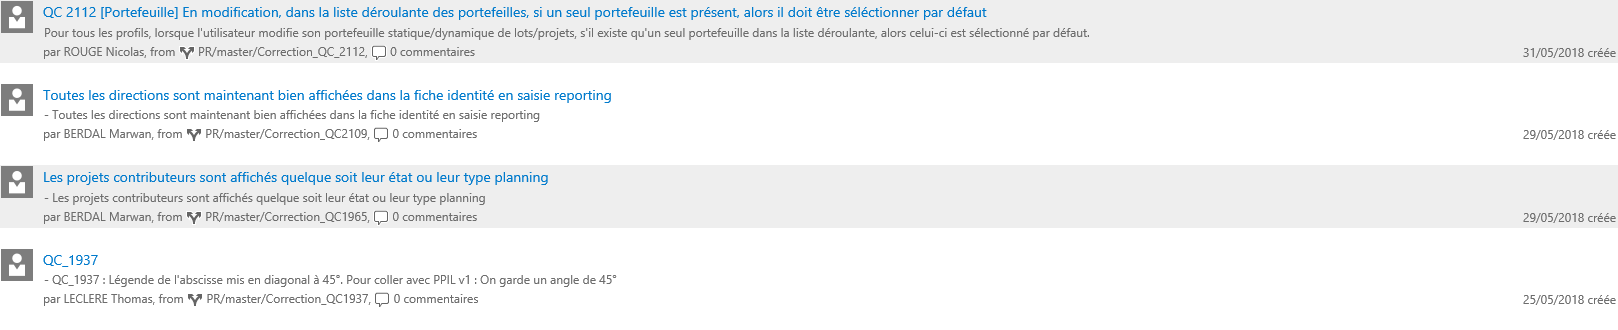
\includegraphics[width=1\textwidth]{images/PullRequest.png}
\caption{Visual Studio Team Foundation : Les Pull Request}
\end{figure}

Ci-dssous le workflow des anomalies dans HPALM :
\begin{figure}[!h]
\centering
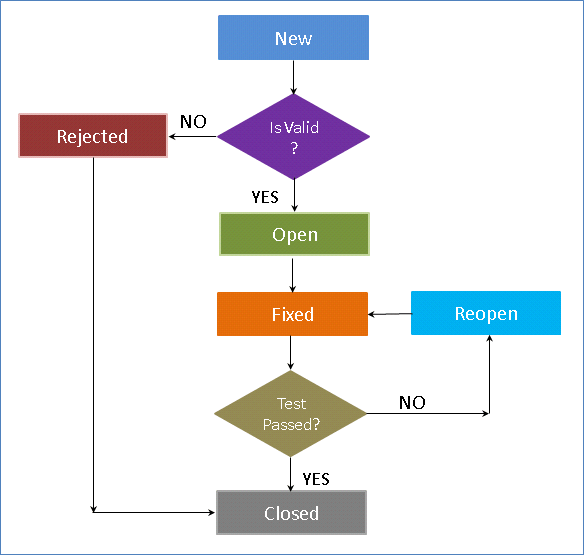
\includegraphics[width=0.6\textwidth]{images/DefectHPALM.png}
\caption{HPALM : Defect Workflow}
\end{figure}

\subsection{Quelques exemples d'anomalies corrigées}

Toutes les anomalies ont été intéressantes à corriger. Elles m'ont fait progresser et travailler sur des technologies diverses. J'ai réussi à acquérir les compétences techniques et nécessaires au projet. L'enjeu de la correction de ces anomalies : aucun retour bloquant en qualification interne et externe tout en garantissant la non régression.

\subsubsection{Anomalie [Portefeuille][liste déroulante]}

Visuel de l'anomalie dans HPALM :
\begin{figure}[!h]
\centering
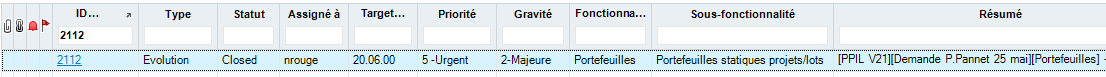
\includegraphics[width=1\textwidth]{images/QC2120.PNG}
\caption{HPALM : Defect 2112}
\end{figure}

On peut voir que l'anomalie est de priorité "urgente" et de gravité "majeure". Elle a été détectée par le client (priorité supplémentaire).

\textbf{Description de la correction à effectuer :} 

[Profil CP ou Manager][portefeuille]
Dans la liste déroulante qui apparaît lorsqu'on veut ajouter des projets ou des lots dans les différents portefeuilles de : 
\begin{itemize}
    \item lots statiques,
    \item lots dynamiques,
    \item projets statiques,
    \item projets dynamiques.
\end{itemize}

Sélectionner par défaut un portefeuille s'il n'y en a qu'un seul. Ne rien sélectionner par défaut sinon. 
[Profil Responsable DSI][portefeuille], Sélectionner par défaut "Mes projets favoris" quel que soit le nombre de portefeuilles existants.

Avant de commencer la correction du code de cette anomalie, j'ai alerté le référent technique : la description de l'anomalie était sujette à interprétation. Le RT a remonté l'information au client, qui a fait un retour en précisant l'anomalie.

Lors de la correction en elle-même, j'ai identifié où faire les modifications de code. Puis au cours de celle-ci, j'ai pu monter en compétence sur du C\#, du Type Script ainsi que le framework Kendo. J'ai pris en compte les différentes conditions pour réaliser les différentes actions correctrices. 

\begin{figure}[!h]
\centering
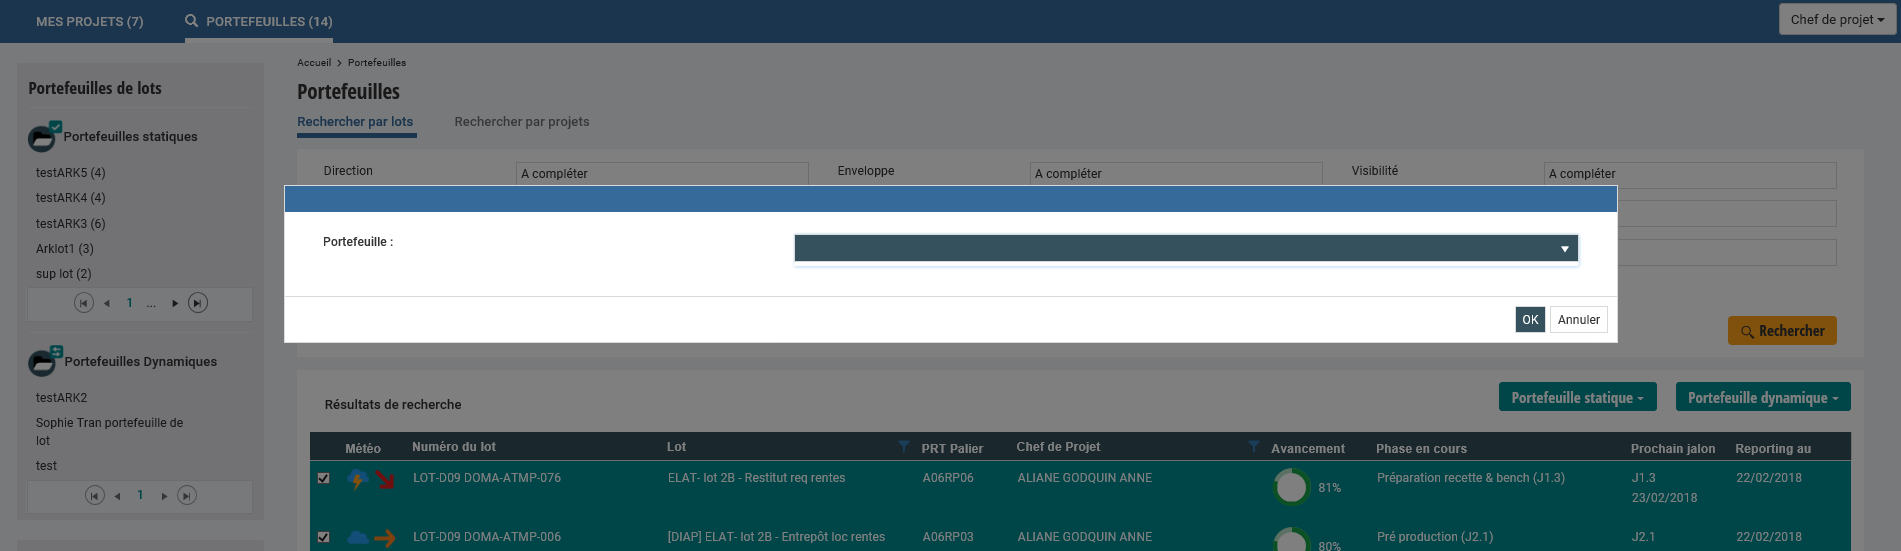
\includegraphics[width=1\textwidth]{images/correction1.PNG}
\caption{HPALM : Defect 2112}
\end{figure}

\subsubsection{Anomalie [Suppression des lots non effective dans plusieurs cas]}

\textbf{Description de la correction à effectuer :} 
La suppression des lots est non effective selon certains critères :
\begin{itemize}
    \item Un lot ne se supprime pas quand il est dans un portefeuille (le lot se supprime visuellement mais pas en base de donnée, quand on refresh la page il réapparaît) ;
    \item Un lot ne se supprime pas quand il a des demandes rattachées ;
    \item Un lot ne se supprime pas quand il n'a pas de projet de référence.
\end{itemize}

Cette anomalie m'a pris plusieurs jours de correction, les points importants à souligner sont : 
\begin{itemize}
    \item Il a fallu mettre en place plusieurs jeux de données pour visualiser l'anomalie ;
    \item Pendant la correction, j'ai détecté une autre anomalie : un lot sans projet de référence ne s'affiche pas dans un portefeuille (Anomalie que j'ai corrigée par la suite) ;
    \item J'ai proposé une solution efficace et correcte ;
    \item Je suis allé voir Nicolas (le RT du projet), afin d'avoir son retour sur ma correction ;
    \item Il m'a apporté son recul et son expérience. Il m'a proposé de refaire une partie de cette correction en modifiant une procédure stockée en SQL plutôt que de modifier une partie du code. Cette solution étant préférable pour la maintenir le code et l'optimiser.
\end{itemize}

\subsubsection{Anomalie [Onglet synthèse]}

\textbf{Description de l'anomalie :} En restitution d'un projet, onglet synthèse, quand on remonte sur une semaine précédente, les dates ne sont pas les bonnes. 

\begin{figure}[!h]
\centering
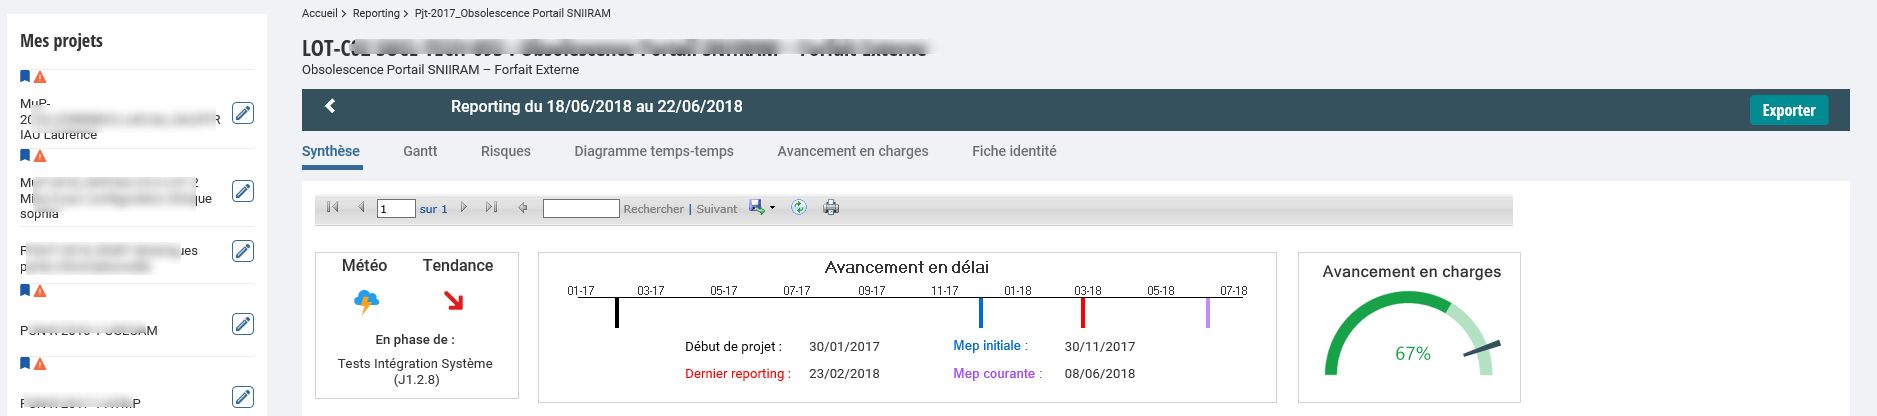
\includegraphics[width=1\textwidth]{images/ppil-indicateur-synthese-censored.png}
\caption{Indicateur Synthèse}
\end{figure}

Les difficultés rencontrées lors de cette correction ont été :
\begin{itemize}
    \item Comprendre le fonctionnel, c'est-à-dire la logique des jalons.
    \item Travailler et modifier des requêtes complexes.
    \item Ne pas faire de régression.
\end{itemize}


\subsubsection{L'indicateur Capacity Planning : des expressions multidimensionnelles}

Le Capacity Planning est sans doute l'indicateur le plus complexe de PPIL. En effet, le Capacity Planning récupère les données grâce à des expressions multidimensionnelles (MDX) (Multidimensional Expressions), un langage de requête pour les bases de données OLAP. Je dois donc manipuler des expressions multidimensionnelles afin d'extraire des données stockées dans le Cube. Aucun membre de l'équipe est expert dans cette technologie. J'ai donc adoptée une démarche d'analyse du fonctionnement des requêtes/expressions existantes et montée en compétence sur les bases de données OLAP. Pour le moment, j'ai réussi à corriger une des trois anomalies qui m'ont été confiés. Vous pouvez trouver en annexes une image du Capacity Planning.

%%% Local Variables: 
%%% mode: latex
%%% TeX-master: "isae-report-template"
%%% End: 